%\VignetteEngine{knitr::knitr}
%\VignetteDepends{investr}
%\VignetteDepends{drc}
%\VignetteDepends{car}
%\VignetteDepends{boot}
%\VignetteIndexEntry{Introduction to investr}
\documentclass[a4paper]{report}\usepackage[]{graphicx}\usepackage[]{color}
%% maxwidth is the original width if it is less than linewidth
%% otherwise use linewidth (to make sure the graphics do not exceed the margin)
\makeatletter
\def\maxwidth{ %
  \ifdim\Gin@nat@width>\linewidth
    \linewidth
  \else
    \Gin@nat@width
  \fi
}
\makeatother

\definecolor{fgcolor}{rgb}{0.345, 0.345, 0.345}
\newcommand{\hlnum}[1]{\textcolor[rgb]{0.686,0.059,0.569}{#1}}%
\newcommand{\hlstr}[1]{\textcolor[rgb]{0.192,0.494,0.8}{#1}}%
\newcommand{\hlcom}[1]{\textcolor[rgb]{0.678,0.584,0.686}{\textit{#1}}}%
\newcommand{\hlopt}[1]{\textcolor[rgb]{0,0,0}{#1}}%
\newcommand{\hlstd}[1]{\textcolor[rgb]{0.345,0.345,0.345}{#1}}%
\newcommand{\hlkwa}[1]{\textcolor[rgb]{0.161,0.373,0.58}{\textbf{#1}}}%
\newcommand{\hlkwb}[1]{\textcolor[rgb]{0.69,0.353,0.396}{#1}}%
\newcommand{\hlkwc}[1]{\textcolor[rgb]{0.333,0.667,0.333}{#1}}%
\newcommand{\hlkwd}[1]{\textcolor[rgb]{0.737,0.353,0.396}{\textbf{#1}}}%

\usepackage{framed}
\makeatletter
\newenvironment{kframe}{%
 \def\at@end@of@kframe{}%
 \ifinner\ifhmode%
  \def\at@end@of@kframe{\end{minipage}}%
  \begin{minipage}{\columnwidth}%
 \fi\fi%
 \def\FrameCommand##1{\hskip\@totalleftmargin \hskip-\fboxsep
 \colorbox{shadecolor}{##1}\hskip-\fboxsep
     % There is no \\@totalrightmargin, so:
     \hskip-\linewidth \hskip-\@totalleftmargin \hskip\columnwidth}%
 \MakeFramed {\advance\hsize-\width
   \@totalleftmargin\z@ \linewidth\hsize
   \@setminipage}}%
 {\par\unskip\endMakeFramed%
 \at@end@of@kframe}
\makeatother

\definecolor{shadecolor}{rgb}{.97, .97, .97}
\definecolor{messagecolor}{rgb}{0, 0, 0}
\definecolor{warningcolor}{rgb}{1, 0, 1}
\definecolor{errorcolor}{rgb}{1, 0, 0}
\newenvironment{knitrout}{}{} % an empty environment to be redefined in TeX

\usepackage{alltt}
\usepackage[utf8]{inputenc}
\usepackage[T1]{fontenc}
\usepackage{RJournal}
\usepackage{amsmath,amssymb,array}
\usepackage{booktabs}

%% load any required packages here
\IfFileExists{upquote.sty}{\usepackage{upquote}}{}
\begin{document}

%% do not edit, for illustration only
\sectionhead{Contributed research article}
\volume{6}
\volnumber{1}
\year{2014}
\month{June}

\begin{article}

\title{\pkg{investr}: An R Package for Inverse Estimation}
\author{by Brandon M. Greenwell and Christine M. Schubert Kabban}

\maketitle



\abstract{
Inverse estimation is a classical and well-known problem in regression. In simple terms, it involves the use of an observed value of the response to make inference on the corresponding unknown value of the explanatory variable. To our knowledge, however, statistical software is somewhat lacking the capabilities for analyzing these types of problems. In this paper\footnote{The views expressed in this paper are those of the authors, and do not reflect the official policy or position of the United States Air Force, Navy, Department of Defense, or the U.S. Government.}, we introduce \CRANpkg{investr} (which stands for \textbf{inv}erse \textbf{est}imation in \textbf{R}), a package for solving inverse estimation problems in both linear and nonlinear regression models.
}

\section{Introduction}
Consider the regression model $\mathcal{Y}_i = f\left( x_i; \boldsymbol{\beta} \right) + \epsilon_i$ $(i = 1, \dotsc, n)$, where $f$ is a known expectation function (called a \dfn{calibration curve}) that is monotonic over the range of interest and $\epsilon_i \stackrel{iid}{\sim} \mathcal{N}\left( 0, \sigma^2 \right)$. A common problem in regression is to predict a future response $\mathcal{Y}_0$ from a known value of the explanatory variable $x_0$. Often, however, there is a need to do the reverse; that is, given an observed value of the response $\mathcal{Y} = y_0$, estimate the unknown value of the explanatory variable $x_0$. This is known as the \dfn{calibration problem}, though we refer to it more generally as inverse estimation. In this paper, we consider only \dfn{controlled calibration}, where the values of the explanatory variables are fixed by design. A more thorough overview of the calibration problem, including Bayesian approaches and multivariate calibration, is given in \citet{osborne-statistical-1991}.

There are three main functions available in the \pkg{investr} package:
\begin{itemize}
  \item \code{calibrate};
  \item \code{invest};
  \item \code{plotFit}.
\end{itemize}
\code{calibrate} operates on objects of class \code{lm} and can only be used when the expectation function has the form $f(x_i; \boldsymbol{\beta}) = \beta_0 + \beta_1 x_i$ (i.e., the simple linear regression model), where closed-form solutions are available for calculating confidence intervals for $x_0$. For more complicated models (e.g., polynomial and nonlinear regression), closed-form expressions are usually not available and iterative techniques will be required. This is the purpose of the  function \code{invest}, which calculates the point estimate and confidence intervals for $x_0$ by calling the function \code{uniroot} from the \pkg{stats} package. The function \code{plotFit} produces a scatterplot of the data with fitted regression curve and the option to add confidence/prediction bands for the response (pointwise or adjusted). It can be used with single-predictor objects of class \code{lm} or \code{nls}; however, for objects of class \code{nls}, confidence/prediction bands are based on the linear approximation and can be misleading \citep[pg. 65]{bates-nonlinear-1988}. The development version of \pkg{investr} can be found on GitHub at \url{https://github.com/w108bmg/investr}.  To report bugs or issues, contact the main author or submit them to \url{https://github.com/w108bmg/investr/issues}.
and can easily be installed using the the \pkg{devtools} package \citep{hadley-devtools-2013}:
\begin{knitrout}
\definecolor{shadecolor}{rgb}{0.969, 0.969, 0.969}\color{fgcolor}\begin{kframe}
\begin{alltt}
\hlcom{# Install development version from GitHub}
\hlkwd{install.packages}\hlstd{(}\hlstr{"devtools"}\hlstd{)}
\hlstd{devtools}\hlopt{::}\hlkwd{install_github}\hlstd{(}\hlkwc{repo} \hlstd{=} \hlstr{"bgreenwell/investr"}\hlstd{)}
\end{alltt}
\end{kframe}
\end{knitrout}


\section{Calibration for straight line regression}

Consider the most common calibration model, $\mathcal{Y}_i = \beta_0 + \beta_1 x_i + \epsilon_i$ $(i = 1, \dotsc, n)$, where $x_i$ is fixed and $\epsilon_i \stackrel{iid}{\sim} \mathcal{N}\left( 0, \sigma^2 \right)$. Suppose we obtain a series of $m$ observations $y_{01}, \dotsc, y_{0m}$ which are associated with the same (unknown) $x_0$. It can be shown \citep{graybill-theory-1976} that the maximum likelihood (ML) estimator of $x_0$, also known as the \dfn{classical estimator}, is
\begin{equation}
\label{eqn:x0-mle}
  \widehat{x}_0 = \frac{\bar{y}_0 - \widehat{\beta}_0}{\widehat{\beta}_1},
\end{equation}
where $\widehat{\beta}_0$ and $\widehat{\beta}_1$ are the usual ML estimators of $\beta_0$ and $\beta_1$, respectively, and $\bar{y}_0 = \sum_{j = 1}^m y_{0j}/m$. The classical estimator in general is computed as $\widehat{x}_0 = f^{-1}\left( \bar{y}_0; \widehat{\boldsymbol{\beta}} \right)$; that is, by inverting the fitted calibration curve at $\bar{y}_0$ \citep{eisenhart-interpretation-1939}. Since $\widehat{x}_0$ is a ratio of jointly normal random variables, it is not surprising to learn that it does not have any finite moments (think of a standard Cauchy distribution). The sampling distribution of $\widehat{x}_0$ is complicated, but fortunately, not required for setting an exact $100(1 - \alpha)\%$ confidence interval on $x_0$. This is discussed in the next section. 

\subsection{Inversion interval}
\label{sec:inversion}

It can be shown (see, for example, \citet[pp. 47-51]{draper-applied-1998}) that an exact $100(1 - \alpha)\%$ confidence interval for $x_0$ is given by
\begin{equation}
\label{eqn:x0-inversion-interval}
  \widehat{x}_0 + \frac{\left( \widehat{x}_0 - \bar{x} \right)g \pm \left( t\widehat{\sigma}/\widehat{\beta}_1 \right)\sqrt{\left( \widehat{x}_0 - \bar{x} \right)^2 / S_{xx} + (1 - g)\left( \frac{1}{m} + \frac{1}{n} \right)}}{1 - g},
\end{equation}
where $S_{xx} = \sum_{i = 1}^{n}\left(x_i - \bar{x}\right)^2$, $g = \left( t^2 \widehat{\sigma}^2 \right) / \left( \widehat{\beta}_1^2 S_{xx} \right)$ and $t = t_{\alpha/2, n + m - 3}$ is the upper $1 - \alpha$ percentile of a Student's $t$-distribution with $n + m - 3$ degrees of freedom. The inversion interval \eqref{eqn:x0-inversion-interval} can also be obtained using a fiducial argument, as in \citet{fieller-some-1954}.  For the special case $m = 1$, the inversion interval is equivalent to inverting a $100(1 - \alpha)\%$ prediction interval for the response. In other words, if one draws a horizontal line through a scatterplot of the data at $y_0$, then the abscissas of its intersection with the usual (pointwise) prediction band for $f$ correspond to the endpoints of the inversion interval \eqref{eqn:x0-inversion-interval}.  This interval should only be used when the usual $\mathcal{F}$ test for testing $\mathcal{H}_0: \beta_1 = 0$ versus $\mathcal{H}_1: \beta_1 \ne 0$ can be rejected at the specified $\alpha$ level; in other words, when the regression line is not "too" flat.  If $\mathcal{H}_0$ is not rejected, then such a confidence interval for $x_0$ may result in either the entire real line or two semi-infinite intervals \citep[p. 429]{graybill_regression_1994} --- see Figure~\ref{fig:bands}.  The \code{plotFit} function in the \pkg{investr} package can be used for drawing scatterplots with the fitted model and confidence/prediction bands. To calculate the inversion interval for the linear calibration problem, we use the \code{calibrate} function and specify the option \code{interval = "inversion"} (the default) as in the following example.

The data frame \code{arsenic} contains the true amounts of arsenic present in 32 water samples \citep{graybill_regression_1994}. Also present, is the amount of arsenic measured by some field test, which is subject to error. A new water sample is obtained and subjected the field test producing a reading of 3.0 $\mu$g/ml. It is desired to infer the true amount of arsenic present in the sample. The following code fits a simple linear regression model to the arsenic data and then uses the \code{calibrate} function to compute the ML estimate and corresponding 90\% calibration interval based on Equation~\eqref{eqn:x0-inversion-interval}.
\begin{knitrout}
\definecolor{shadecolor}{rgb}{0.969, 0.969, 0.969}\color{fgcolor}\begin{kframe}
\begin{alltt}
\hlkwd{library}\hlstd{(investr)}
\hlstd{mod} \hlkwb{<-} \hlkwd{lm}\hlstd{(measured} \hlopt{~} \hlstd{actual,} \hlkwc{data} \hlstd{= arsenic)}
\hlstd{(res} \hlkwb{<-} \hlkwd{calibrate}\hlstd{(mod,} \hlkwc{y0} \hlstd{=} \hlnum{3}\hlstd{,} \hlkwc{interval} \hlstd{=} \hlstr{"inversion"}\hlstd{,} \hlkwc{level} \hlstd{=} \hlnum{0.9}\hlstd{))}
\end{alltt}
\begin{verbatim}
## estimate    lower    upper 
## 2.931449 2.603537 3.258658
\end{verbatim}
\begin{alltt}
\hlcom{# Figure 1}
\hlkwd{plotFit}\hlstd{(mod,} \hlkwc{interval} \hlstd{=} \hlstr{"prediction"}\hlstd{,} \hlkwc{level} \hlstd{=} \hlnum{0.9}\hlstd{,} \hlkwc{shade} \hlstd{= T,}
        \hlkwc{col.pred} \hlstd{=} \hlstr{"skyblue"}\hlstd{)}
\hlkwd{abline}\hlstd{(}\hlkwc{h} \hlstd{=} \hlnum{3}\hlstd{,} \hlkwc{v} \hlstd{=} \hlkwd{c}\hlstd{(res}\hlopt{$}\hlstd{lower, res}\hlopt{$}\hlstd{estimate, res}\hlopt{$}\hlstd{upper),} \hlkwc{lty} \hlstd{=} \hlnum{2}\hlstd{)}
\end{alltt}
\end{kframe}\begin{figure}
\includegraphics[width=\maxwidth]{figure/arsenic-plotFit-1} \caption[Scatterplot of the arsenic data with fitted calibration line and pointwise prediction band]{Scatterplot of the arsenic data with fitted calibration line and pointwise prediction band. A horizontal reference line is drawn through the observed value $y_0 = 3$. The vertical lines identify the position of the point estimate and 90\% confidence bounds for $x_0$.}\label{fig:arsenic-plotFit}
\end{figure}


\end{knitrout}
Running the above block of code produces Figure~\ref{fig:arsenic-plotFit} and the following output to the R console:
\begin{example}
  estimate    lower    upper 
    2.9314   2.6035   3.2587
\end{example}
where \code{estimate} is the ML estimate \eqref{eqn:x0-mle}, and \code{lower}/\code{upper} correspond to the lower/upper bounds of the 90\% inversion interval for $x_0$ \eqref{eqn:x0-inversion-interval}. If instead the new water sample was subjected to the field test three times, thereby producing three response values corresponding to $x_0$, say 3.17, 3.09, and 3.16 $\mu$g/ml, we would simply supply \code{calibrate} with a vector of these values as in 
\begin{knitrout}
\definecolor{shadecolor}{rgb}{0.969, 0.969, 0.969}\color{fgcolor}\begin{kframe}
\begin{alltt}
\hlkwd{calibrate}\hlstd{(mod,} \hlkwc{y0} \hlstd{=} \hlkwd{c}\hlstd{(}\hlnum{3.17}\hlstd{,} \hlnum{3.09}\hlstd{,} \hlnum{3.16}\hlstd{),} \hlkwc{interval} \hlstd{=} \hlstr{"inversion"}\hlstd{,} \hlkwc{level} \hlstd{=} \hlnum{0.9}\hlstd{)}
\end{alltt}
\begin{verbatim}
## estimate    lower    upper 
## 3.073191 2.884300 3.261588
\end{verbatim}
\end{kframe}
\end{knitrout}
If \code{interval = "inversion"}, and the slope of the model is not ignificant at the specified $\alpha$ level, then finite confidence limits for $x_0$ will not be produced.  For example, suppose \code{badfit} is an \code{lm} object for which the slope is not significant at the $\alpha = 0.1$ level.  Then, as illustrated in Figure~\ref{fig:bands},
\begin{knitrout}
\definecolor{shadecolor}{rgb}{0.969, 0.969, 0.969}\color{fgcolor}\begin{kframe}
\begin{alltt}
\hlkwd{calibrate}\hlstd{(badfit,} \hlkwc{y0} \hlstd{=} \hlnum{10}\hlstd{,} \hlkwc{level} \hlstd{=} \hlnum{0.9}\hlstd{)}
\end{alltt}
\end{kframe}
\end{knitrout}
will either produce two semi-infinite intervals, e.g.,
\begin{example}
   Error: The calibration line is not well determined.
  Returning two semi-infinite intervals:
  ( -Inf , -282.0006 ) and ( 393.1267 , Inf ) 
\end{example}
or the entire real line, e.g.,
\begin{example}
  estimate    lower    upper 
  -97.5987     -Inf      Inf 
  Warning message:
  The calibration line is not well determined.
\end{example}

% \begin{figure}[htbp]
%   \centering
%   \includegraphics[width = \textwidth]{arsenic-plotFit}
%   \caption{Scatterplot of the arsenic data with fitted calibration line and pointwise prediction band. A horizontal reference line is drawn through the observed value $y_0 = 3$. The vertical lines identify the position of the point estimate and 90\% confidence bounds for $x_0$.}
%   \label{fig:arsenic-plotFit}
% \end{figure}

\begin{knitrout}
\definecolor{shadecolor}{rgb}{0.969, 0.969, 0.969}\color{fgcolor}\begin{figure}
\includegraphics[width=\maxwidth]{figure/bands-1} \caption{Hypothetical $1-\alpha$ (pointwise) prediction bands. \textit{Left}: Horizontal line at $y_0$ intersects the prediction band at two points, resulting in a finite interval. 	extit{Middle}: Horizontal line at $y_0$ does not intersect the prediction band at all resulting in an infinite interval. \textit{Right}: Horizontal line at $y_0$ only intersects with one side of the prediction band resulting in two semi-infinite intervals.}\label{fig:bands}
\end{figure}


\end{knitrout}
% \begin{figure}[htbp]
%   \centering
%   \includegraphics[width = \textwidth]{bands}
%   \caption{Hypothetical $1-\alpha$ (pointwise) prediction bands. \textit{Left}: Horizontal line at $y_0$ intersects the prediction band at two points, resulting in a finite interval. \textit{Middle}: Horizontal line at $y_0$ does not intersect the prediction band at all resulting in an infinite interval. \textit{Right}: Horizontal line at $y_0$ only intersects with one side of the prediction band resulting in two semi-infinite intervals.}
%   \label{fig:bands}
% \end{figure}

\subsection{Wald interval}

Another common approach to computing calibration intervals is to use the delta method \citep{dorfman-note-1938}. It is easy to show that an approximate standard error for the ML estimator \eqref{eqn:x0-mle}, based on a first-order Taylor series approximation, is given by
\begin{equation}
\label{eqn:x0-se}
  \widehat{\mathrm{se}}\left( \widehat{x}_0 \right) = \frac{\widehat{\sigma}}{\left| \widehat{\beta}_1 \right|} \sqrt{\frac{1}{m} + \frac{1}{n} + \frac{\left( \widehat{x}_0 - \bar{x} \right)^2}{S_{xx}}}.
\end{equation}
Assuming large sample normality for $\widehat{x}_0$ leads to an approximate $100(1 - \alpha)\%$ Wald confidence interval for $x_0$ of
\begin{equation}
\label{eqn:x0-wald-interval}
  \widehat{x}_0 \pm t_{\alpha/2, n+m-3} \frac{\widehat{\sigma}}{\left| \widehat{\beta}_1 \right|} \sqrt{\frac{1}{m} + \frac{1}{n} + \frac{\left( \widehat{x}_0 - \bar{x} \right)^2}{S_{xx}}}.
\end{equation}
This is equivalent to taking $g = 0$ in the inversion interval \eqref{eqn:x0-inversion-interval}. Unlike the inversion interval, though, the Wald interval always exists and is symmetric about $\widehat{x}_0$. This symmetry is attractive, but not always realistic, such as when the calibration curve $f$ is nonlinear and has horizontal asymptotes. To obtain a Wald-type interval we specify \code{interval = "Wald"} in the call to \code{calibrate}. For instance,
\begin{knitrout}
\definecolor{shadecolor}{rgb}{0.969, 0.969, 0.969}\color{fgcolor}\begin{kframe}
\begin{alltt}
\hlkwd{calibrate}\hlstd{(mod,} \hlkwc{y0} \hlstd{=} \hlnum{3}\hlstd{,} \hlkwc{interval} \hlstd{=} \hlstr{"Wald"}\hlstd{,} \hlkwc{level} \hlstd{=} \hlnum{0.9}\hlstd{)}
\end{alltt}
\begin{verbatim}
##  estimate     lower     upper        se 
## 2.9314491 2.6039901 3.2589080 0.1929338
\end{verbatim}
\end{kframe}
\end{knitrout}
produces the output
\begin{example}
  estimate    lower    upper       se 
    2.9314   2.6040   3.2589   0.1929
\end{example}
The point estimate remains unchanged (as expected) but the calibration interval is slightly different. The major benefit of using the delta method to compute calibration intervals is that it always exists and provides us with an asymptotic estimate of the standard error, which in this case $\widehat{\mathrm{se}} = 0.1929$. The bootstrap, as discussed in Section~\ref{sec:bootstrap}, also provides calibration intervals and an estimate of the standard error, but does not require large samples or specific distribution assumptions.

\subsection{Confidence interval for a specified mean response}

Instead of inferring the value of $x_0$ that corresponds to an observed value of the response $y_0$, suppose we want to infer the value of $x_0$ that %corresponds to a specified mean response $\mathrm{E}(\mathcal{Y}_0) = \mu_0$. The obvious ML estimate of $x_0$ is
corresponds to a specified value of the mean response, say $f\left( x_0; \boldsymbol{\beta} \right) = \mu_0$. The obvious ML estimate of $x_0$ is
\begin{equation}
\label{eqn:x0-mle-regulation}
  \widehat{x}_0 = \frac{\mu_0 - \widehat{\beta}_0}{\widehat{\beta}_1},
\end{equation}
which is the same as Equation~\eqref{eqn:x0-mle} but with $\bar{y}_0$ replaced with $\mu_0$, a fixed population parameter. This is analogous to the difference between (i) predicting a future value of the response corresponding to a given value of the explanatory variable and (ii) estimating the mean response that corresponds to a particular value of the explanatory variable. Thus, the point estimates \eqref{eqn:x0-mle} and \eqref{eqn:x0-mle-regulation} are the same but the former has greater variability inherited from the variance of $\overline{\mathcal{Y}}_0$.  This is sometimes referred to as \dfn{regulation} (as opposed to calibration) and is described in more detail in \citet[chap. 6]{graybill_regression_1994}. The confidence interval formulas for $x_0$ corresponding to a specified mean response (i.e., regulation) are the same as those given in Equations~\eqref{eqn:x0-inversion-interval} and \eqref{eqn:x0-wald-interval}, but with $1/m = 0$ and $t_{\alpha/2, n + m - 3}$ replaced with $t_{\alpha/2, n - 2}$. %For instance, the Wald interval in regulation is simply
For instance, the Wald interval for $x_0$ corresponding to $\mu_0$ is simply
\begin{equation*}
  \widehat{x}_0 \pm  t_{\alpha/2, n - 2}\frac{\widehat{\sigma}}{\left| \widehat{\beta}_1 \right|} \sqrt{\frac{1}{n} + \frac{\left( \widehat{x}_0 - \bar{x} \right)^2}{S_{xx}}},
\end{equation*}

where $\widehat{x}_0$ is calculated as in Equation~\eqref{eqn:x0-mle-regulation}.  To obtain calibration intervals corresponding to a specified mean response, %(rather than an observed response), 
use the option \code{mean.response = TRUE}. 

To illustrate, consider the crystal growth data taken from \citet[pg. 119]{graybill_regression_1994}. These data are from an experiment in which the weight in grams of 14 crystals were recorded after letting the crystals grow for different (predetermined) amounts of time in hours. The weight of each crystal is plotted against time in Figure~\ref{fig:crystal-plotFit}. Suppose we want to estimate the growth time in hours that corresponds to an average weight of 8 grams; that is, we want to estimate $x_0$ corresponding to $\mu_0 = 8$. The following code chunk fits a simple linear regression model to the crystal growth data and then computes the ML estimate and a 95\% calibration interval for $x_0$.
\begin{knitrout}
\definecolor{shadecolor}{rgb}{0.969, 0.969, 0.969}\color{fgcolor}\begin{kframe}
\begin{alltt}
\hlstd{mod} \hlkwb{<-} \hlkwd{lm}\hlstd{(weight} \hlopt{~} \hlstd{time,} \hlkwc{data} \hlstd{= crystal)}
\hlstd{(res} \hlkwb{<-} \hlkwd{calibrate}\hlstd{(mod,} \hlkwc{y0} \hlstd{=} \hlnum{8}\hlstd{,} \hlkwc{mean.response} \hlstd{= T))}
\end{alltt}
\begin{verbatim}
## estimate    lower    upper 
## 15.88820 14.65896 17.15963
\end{verbatim}
\begin{alltt}
\hlcom{# Figure 3}
\hlkwd{plotFit}\hlstd{(mod,} \hlkwc{interval} \hlstd{=} \hlstr{"confidence"}\hlstd{,} \hlkwc{pch} \hlstd{=} \hlnum{19}\hlstd{,} \hlkwc{shade} \hlstd{= T,}
        \hlkwc{col.conf} \hlstd{=} \hlstr{"plum"}\hlstd{,} \hlkwc{extend.range} \hlstd{= T)}
\hlkwd{abline}\hlstd{(}\hlkwc{h} \hlstd{=} \hlnum{8}\hlstd{,} \hlkwc{v} \hlstd{=} \hlkwd{c}\hlstd{(res}\hlopt{$}\hlstd{lower, res}\hlopt{$}\hlstd{estimate, res}\hlopt{$}\hlstd{upper),} \hlkwc{lty} \hlstd{=} \hlnum{2}\hlstd{)}
\end{alltt}
\end{kframe}\begin{figure}
\includegraphics[width=\maxwidth]{figure/crystal-plotFit-1} \caption[Scatterplot of the crystal growth data with fitted calibration line and pointwise confidence band]{Scatterplot of the crystal growth data with fitted calibration line and pointwise confidence band. A horizontal reference line is drawn at $\mu_0 = 8$. The vertical lines identify the position of the point estimate and 95\% confidence bounds for the growth time $x_0$.}\label{fig:crystal-plotFit}
\end{figure}


\end{knitrout}
The output for this code chunk should be
\begin{example}
  estimate    lower    upper 
   15.8882  14.6590  17.1596 
\end{example}
Thus, in order to produce crystals with an average weight of 8 grams, they should be grown for an estimated 15.8882 hours. A 95\% confidence interval for the growth time is (14.6590,  17.1596).  Obviously, if \code{mean.response = TRUE}, then \code{y0} can only take a single value; otherwise, an error will be displayed as in the following:
\begin{knitrout}
\definecolor{shadecolor}{rgb}{0.969, 0.969, 0.969}\color{fgcolor}\begin{kframe}
\begin{alltt}
\hlkwd{calibrate}\hlstd{(mod,} \hlkwc{y0} \hlstd{=} \hlkwd{c}\hlstd{(}\hlnum{8}\hlstd{,} \hlnum{9}\hlstd{),} \hlkwc{mean.response} \hlstd{= T)}
\end{alltt}


{\ttfamily\noindent\bfseries\color{errorcolor}{\#\# Error in calibrate.default(cbind(x, y), ...): Only one mean response value allowed.}}\end{kframe}
\end{knitrout}
which displays the message
\begin{example}
  Error in calibrate.default(cbind(x, y), ...) : 
    Only one mean response value allowed.
\end{example}

% \begin{figure}[htbp]
%   \centering
%   \includegraphics[width = \textwidth]{crystal-plotFit}
%   \caption{Scatterplot of the crystal growth data with fitted calibration line and pointwise confidence band. A horizontal reference line is drawn at $\mu_0 = 8$. The vertical lines identify the position of the point estimate and 95\% confidence bounds for the growth time $x_0$.}
%   \label{fig:crystal-plotFit}
% \end{figure}

%For example,
%\begin{example}
%  calibrate(mod, y0 = 3, interval = "inversion", level = 0.9, mean.response = T)
%\end{example}
%produces a ML estimate of 2.9314 and a 90\% inversion interval of (2.8724, 2.9898), much smaller compared to the interval obtained previously. (Think of this as inverting a confidence interval for the mean response as opposed to inverting a prediction interval for an individual response). 

This type of calibration problem is similar to computing the \dfn{median effective dose} ($ED_{0.5}$), or more generally $ED_p$ where $0 < p < 1$, in binary response models. In R, these models are usually fit with the \code{glm} function from the \pkg{stats} package. The function \code{dose.p} from the \CRANpkg{MASS} package \citep{venables-modern-2002} can then be used to compute the ML estimate of $ED_p$ for specified $p$. An estimate of the asymptotic standard error based on the delta method is also given which can be used to calculate a Wald-based confidence interval for $ED_p$. A future release of \pkg{investr} will likely make an inversion-type interval available for these models as well (i.e. by inverting a confidence interval for the mean response on the link scale). The package \CRANpkg{drc} \citep{ritz-bioassay-2005}, for fitting dose-response curves, may also be of interest.

\subsection{Simultaneous calibration intervals}

The calibration intervals discussed so far are one-at-a-time intervals. If $k$ new values of the response are observed that each correspond to a different unknown, say $x_{01}, \dotsc x_{0k}$, then we need to adjust the critical value used in the inversion and Wald intervals accordingly. The simplest approaches are of course, the \dfn{Bonferroni} and \dfn{Scheff\'{e}} procedures. These can be computed by specifying the \code{adjust} option which can take any of the following arguments: \code{"none"} (the default), \code{"bonferroni"}, or \code{"scheffe"}. The value $k$ also needs to be specified. See \citet[chap. 3]{miller-simultaneous-1981} for more details.

\section{Nonlinear and polynomial calibration}
%\section{Nonlinear calibration}

In application, many relationships are nonlinear (e.g., dose-response curves). The classical estimator along with the inversion and Wald intervals can easily be extended to such nonlinear calibration curves. However, classical inference in these models (such as prediction intervals) are based on large samples and linear approximations (see \citet[chap. 2]{bates-nonlinear-1988}). Thus, for nonlinear calibration curves, the inversion interval provides only an approximate $100(1 - \alpha)\%$ confidence interval for $x_0$ as does the Wald interval.  Calibration in nonlinear models is discussed in further detail in \citet{schwenke-calibration-1991}, \citet[pp. 245-250]{seber-nonlinear-2003}, and \citet[chap. 5]{huet-statistical-2004}.  For calibration in polynomial models, see \citet[pp. 47-88]{brown-measurement-1993} and \citet[pg. 172]{seber-linear-2003}.  

The \code{invest} function can be used for inverse estimation with any univariate regression model in R that inherits from class \code{lm} or \code{nls} (with the exception of weighted fits).  For instance, consider the regression model $\mathcal{Y}_i = f\left( x_i; \boldsymbol{\beta} \right) + \epsilon_i$ $(i = 1, \dotsc, n)$, where $f$ may or may not be linear in $\boldsymbol{\theta}$.  If we wish to estimate $x_0$ given an observation $y_0$, then the point estimate $\widehat{x}_0$ is given by solving $y_0 = f\left(x; \widehat{\boldsymbol{\theta}}\right)$ for $x$. The solution will be unique as long as $f$ is monotonic in the region of interest.  The \code{invest} function computes $\widehat{x}_0$ by calling the \pkg{stats} functions \code{predict} and \code{uniroot} to solve
\begin{equation*}
  y_0 - f\left(x; \widehat{\boldsymbol{\theta}}\right) = 0
\end{equation*}
numerically for $x$. %Consequently, if the solution lies outside the range of predictor values, then the user may need to supply a lower and upper bound for which to search for the solution. These can be supplied to \code{invest} through the options \code{lower} and \code{upper}; for details, see the help pages for \code{invest} and \code{uniroot}. 

%\subsection{Approximate inversion interval}
\subsection{Approximate confidence intervals}

Equation~\eqref{eqn:x0-inversion-interval} gives a closed-form expression for the inversion interval for the case of simple linear regression. In more complicated cases, such an expression is not available and the interval must be found numerically. It can be shown (see, for example, \citet[pp. 245-246]{seber-nonlinear-2003}) that 
\begin{equation}
\label{eqn:predictive-pivot}
  \mathcal{T}_{x_0} = \frac{\mathcal{Y}_0 - f\left(x_0; \widehat{\boldsymbol{\theta}}\right)}{\left\{\widehat{\sigma}^2 + \widehat{S}_{x_0}^2\right\}^{1/2}} \stackrel{\cdot}{\sim} t_{n-p},
\end{equation}
where $\widehat{S}_{x_0}^2$ is the estimated variance of $f\left(x_0; \widehat{\boldsymbol{\theta}}\right)$. An approximate $100(1-\alpha)\%$ confidence interval for $x_0$ is then given by the set
\begin{equation}
\label{eqn:inversion}
  \bigg\{ x: t_{\alpha/2, n-p} < \mathcal{T}_x < t_{1-\alpha/2, n-p} \bigg\}.
\end{equation}
Essentially, \code{invest} finds the lower and upper limits for this interval by solving the equations
\begin{equation*}
  \mathcal{T}_x - t_{\alpha/2, n-p} = 0 \quad \text{and} \quad \mathcal{T}_x - t_{1-\alpha/2, n-p} = 0
\end{equation*}
numerically for $x_0$.  For the special case of the simple linear regression model, These limits coincide with Equation~\eqref{eqn:x0-inversion-interval} and the coverage probability is exactly $1-\alpha$.  

\begin{equation*}
 \Pr\left[t_{\alpha/2, n-p} < \mathcal{T} < t_{1-\alpha/2, n-p}\right] \approx 1-\alpha
\end{equation*}

%\subsection{Wald interval}

The Wald interval for $x_0$ is also easily extended. It has the basic form: $\widehat{x}_0 \pm t_{\alpha/2, n-p}\widehat{\mathrm{se}}\left(\widehat{x}_0\right)$, where $p$ is the dimension of $\boldsymbol{\theta}$. The estimated standard error $\widehat{\mathrm{se}}\left(\widehat{x}_0\right)$ is based on a first-order Taylor Series approximation. For the special case of the simple linear regression model, this approximation results in Equation~\eqref{eqn:x0-se}. 

Since the point estimate and confidence intervals for $x_0$ are obtained numerically using \code{uniroot}, \code{invest} has the additional options \code{lower}, \code{upper}, \code{tol}, and \code{maxiter}.  See the reference manual for details.

To get an idea of how \code{invest} works, consider the data in Figure~\ref{fig:sine-plotFit} which were generated from the model $\mathcal{Y} = 5 + x-\sin(x) + 1.5\mathcal{Z}$, where $\mathcal{Z}$ is a standard normal random variable.  Suppose we want to estimate $x_0$ given a new observation, say $y_0 = 22$.  Fitting a model of the form $f(x; \theta) = \theta_1 + \theta_2\left[x-\sin(x)\right]$ to the sample, we obtain $\widehat{f}(x) = 5.490 + 0.941\left[x-\sin(x)\right]$, which is certainly invertible, but $\widehat{f}^{-1}$ cannot be expressed in closed-form using a finite number of terms; thus, $\widehat{x}_0 = \widehat{f}^{-1}(y_0 = 22)$ must be obtained numerically.  The following chunk of code generates the sample data, calculates $\widehat{x}_0$ and an approximate 95\% Wald interval for $x_0$ using the \code{invest} function.  
\begin{knitrout}
\definecolor{shadecolor}{rgb}{0.969, 0.969, 0.969}\color{fgcolor}\begin{kframe}
\begin{alltt}
\hlkwd{set.seed}\hlstd{(}\hlnum{101}\hlstd{)}  \hlcom{# for reproducibility}
\hlstd{x} \hlkwb{<-} \hlkwd{rep}\hlstd{(}\hlkwd{seq}\hlstd{(}\hlkwc{from} \hlstd{=} \hlnum{0}\hlstd{,} \hlkwc{to} \hlstd{=} \hlnum{25}\hlstd{,} \hlkwc{by} \hlstd{=} \hlnum{2}\hlstd{),} \hlkwc{each} \hlstd{=} \hlnum{2}\hlstd{)}
\hlstd{d} \hlkwb{<-} \hlkwd{data.frame}\hlstd{(x,} \hlkwc{y} \hlstd{=} \hlnum{5} \hlopt{+} \hlstd{x} \hlopt{-} \hlkwd{sin}\hlstd{(x)} \hlopt{+} \hlkwd{rnorm}\hlstd{(}\hlkwd{length}\hlstd{(x),} \hlkwc{sd} \hlstd{=} \hlnum{1.5}\hlstd{))}
\hlstd{mod} \hlkwb{<-} \hlkwd{lm}\hlstd{(y} \hlopt{~} \hlkwd{I}\hlstd{(x}\hlopt{-}\hlkwd{sin}\hlstd{(x)),} \hlkwc{data} \hlstd{= d)}
\hlstd{res} \hlkwb{<-} \hlkwd{invest}\hlstd{(mod,} \hlkwc{y0} \hlstd{=} \hlnum{22}\hlstd{,} \hlkwc{interval} \hlstd{=} \hlstr{"Wald"}\hlstd{)}

\hlcom{# Figure 4}
\hlkwd{plotFit}\hlstd{(mod,} \hlkwc{interval} \hlstd{=} \hlstr{"prediction"}\hlstd{,} \hlkwc{shade} \hlstd{=} \hlnum{TRUE}\hlstd{,} \hlkwc{col.pred} \hlstd{=} \hlstr{"seagreen1"}\hlstd{,}
        \hlkwc{extend.range} \hlstd{=} \hlnum{TRUE}\hlstd{)}
\hlkwd{abline}\hlstd{(}\hlkwc{h} \hlstd{=} \hlnum{22}\hlstd{,} \hlkwc{v} \hlstd{= res}\hlopt{$}\hlstd{estimate,} \hlkwc{lty} \hlstd{=} \hlnum{2}\hlstd{)}
\end{alltt}
\end{kframe}\begin{figure}
\includegraphics[width=\maxwidth]{figure/sine-plotFit-1} \caption[Scatterplot of simulated data with fitted calibration line and pointwise prediction band]{Scatterplot of simulated data with fitted calibration line and pointwise prediction band. A horizontal reference line is drawn through the observed value $y_0 = 22$. The vertical line identifies the position of the point estimate $\widehat{x}_0$.}\label{fig:sine-plotFit}
\end{figure}


\end{knitrout}
The point estimate is $\widehat{x}_0 = 16.7053$ with an estimated standard error of 0.8909. The code used by \code{invest} for obtaining the point estimate is essentially
\begin{knitrout}
\definecolor{shadecolor}{rgb}{0.969, 0.969, 0.969}\color{fgcolor}\begin{kframe}
\begin{alltt}
\hlkwd{uniroot}\hlstd{(}\hlkwa{function}\hlstd{(}\hlkwc{x}\hlstd{)} \hlkwd{predict}\hlstd{(mod,} \hlkwc{newdata} \hlstd{=} \hlkwd{list}\hlstd{(}\hlstr{"x"} \hlstd{= x))} \hlopt{-} \hlnum{22}\hlstd{,}
        \hlkwc{lower} \hlstd{=} \hlkwd{min}\hlstd{(d}\hlopt{$}\hlstd{x),} \hlkwc{upper} \hlstd{=} \hlkwd{max}\hlstd{(d}\hlopt{$}\hlstd{x))}\hlopt{$}\hlstd{root}
\end{alltt}
\begin{verbatim}
## [1] 16.70528
\end{verbatim}
\end{kframe}
\end{knitrout}
The code for obtaining the standard error used in the Wald interval is slightly more involved:
\begin{knitrout}
\definecolor{shadecolor}{rgb}{0.969, 0.969, 0.969}\color{fgcolor}\begin{kframe}
\begin{alltt}
\hlcom{# Write x0.hat as function of parameters (theta1.hat, theta2.hat, Y0)}
\hlstd{x0.fun} \hlkwb{<-} \hlkwa{function}\hlstd{(}\hlkwc{params}\hlstd{,} \hlkwc{object} \hlstd{= mod) \{}
  \hlstd{object}\hlopt{$}\hlstd{coefficients} \hlkwb{<-} \hlstd{params[}\hlnum{1}\hlopt{:}\hlnum{2}\hlstd{]}
  \hlkwd{uniroot}\hlstd{(}\hlkwa{function}\hlstd{(}\hlkwc{x}\hlstd{)} \hlkwd{predict}\hlstd{(object,} \hlkwd{list}\hlstd{(}\hlstr{"x"} \hlstd{= x))} \hlopt{-} \hlstd{params[}\hlnum{3}\hlstd{],}
          \hlkwc{lower} \hlstd{=} \hlnum{0}\hlstd{,} \hlkwc{upper} \hlstd{=} \hlnum{25}\hlstd{,} \hlkwc{tol} \hlstd{=} \hlnum{1e-10}\hlstd{)}\hlopt{$}\hlstd{root}
\hlstd{\}}

\hlcom{# Variance-covariance matrix of (theta1.hat, theta2.hat, Y0)'}
\hlstd{covmat} \hlkwb{<-} \hlkwd{diag}\hlstd{(}\hlnum{3}\hlstd{)}
\hlstd{covmat[}\hlnum{1}\hlopt{:}\hlnum{2}\hlstd{,} \hlnum{1}\hlopt{:}\hlnum{2}\hlstd{]} \hlkwb{<-} \hlkwd{vcov}\hlstd{(mod)}
\hlstd{covmat[}\hlnum{3}\hlstd{,} \hlnum{3}\hlstd{]} \hlkwb{<-} \hlkwd{summary}\hlstd{(mod)}\hlopt{$}\hlstd{sigma}\hlopt{^}\hlnum{2}

\hlcom{# Numerically evaluate gradient}
\hlstd{params} \hlkwb{<-} \hlkwd{c}\hlstd{(}\hlkwd{coef}\hlstd{(mod),} \hlkwc{y0} \hlstd{=} \hlnum{22}\hlstd{)}
\hlstd{grad} \hlkwb{<-} \hlkwd{attr}\hlstd{(}\hlkwd{numericDeriv}\hlstd{(}\hlkwd{quote}\hlstd{(}\hlkwd{x0.fun}\hlstd{(params)),} \hlstr{"params"}\hlstd{),} \hlstr{"gradient"}\hlstd{)}

\hlcom{# Calculate standard error}
\hlstd{(se} \hlkwb{<-} \hlkwd{sqrt}\hlstd{(grad} \hlopt \hlstd{covmat} \hlopt \hlkwd{t}\hlstd{(grad)))}
\end{alltt}
\begin{verbatim}
##           [,1]
## [1,] 0.8909255
\end{verbatim}
\end{kframe}
\end{knitrout}
%The interested reader can easily view the package source code at the \href{https://github.com/w108bmg/investr}{GitHub development site} described earlier.

% \begin{figure}[htbp]
%   \centering
%   \includegraphics[width = \textwidth]{sine-plotFit}
%   \caption{Scatterplot of simulated data with fitted calibration line and pointwise prediction band. A horizontal reference line is drawn through the observed value $y_0 = 22$. The vertical line identifies the position of the point estimate $\widehat{x}_0$.}
%   \label{fig:sine-plotFit}
% \end{figure}

The following example uses the nasturtium data from the \pkg{drc} package.  These data were analyzed in \citet{poon-bayesian-1988} using an approximate Bayesian approach.  Bioassays were performed on a type of garden cress called nasturtium.  Six replicates of the response (plant weight in mg after the third week of growth) were measured at seven preselected concentrations of an agrochemical.  The weights corresponding to three new soil samples, all sharing the same (unknown) concentration $x_0$, were observed to be 309, 296, and 419 mg.  The block of code below fits a log-logistic model 
\begin{equation*}
    f(x; \boldsymbol{\theta}) = \left\{ \begin{array}{l l}
                                          \theta_1, &\quad x = 0 \\
                                          \theta_1 / \left[1 + \exp\left\{\theta_2 + \theta_3\ln(x)\right\}\right], &\quad x > 0,
                                        \end{array} \right.
\end{equation*}
and computes an approximate 95\% inversion interval for $x_0$. 
\begin{knitrout}
\definecolor{shadecolor}{rgb}{0.969, 0.969, 0.969}\color{fgcolor}\begin{kframe}
\begin{alltt}
\hlcom{# Load package containing nasturtium data}
\hlkwd{library}\hlstd{(drc)}

\hlcom{# Fit log-logistic model}
\hlstd{mod} \hlkwb{<-} \hlkwd{nls}\hlstd{(weight} \hlopt{~} \hlstd{theta1}\hlopt{/}\hlstd{(}\hlnum{1} \hlopt{+} \hlkwd{exp}\hlstd{(theta2} \hlopt{+} \hlstd{theta3}\hlopt{*}\hlkwd{log}\hlstd{(conc))),}
           \hlkwc{start} \hlstd{=} \hlkwd{list}\hlstd{(}\hlkwc{theta1} \hlstd{=} \hlnum{1000}\hlstd{,} \hlkwc{theta2} \hlstd{=} \hlopt{-}\hlnum{1}\hlstd{,} \hlkwc{theta3} \hlstd{=} \hlnum{1}\hlstd{),}
           \hlkwc{data} \hlstd{= nasturtium)}
\hlkwd{plotFit}\hlstd{(mod,} \hlkwc{interval} \hlstd{=} \hlstr{"prediction"}\hlstd{)} \hlcom{# figure not shown}
\hlcom{# Compute approximate 95% inversion interval}
\hlkwd{invest}\hlstd{(mod,} \hlkwc{y0} \hlstd{=} \hlkwd{c}\hlstd{(}\hlnum{309}\hlstd{,} \hlnum{296}\hlstd{,} \hlnum{419}\hlstd{),} \hlkwc{interval} \hlstd{=} \hlstr{"inversion"}\hlstd{)}
\end{alltt}
\begin{verbatim}
## estimate    lower    upper 
## 2.263854 1.772244 2.969355
\end{verbatim}
\end{kframe}
\end{knitrout}
The interval obtained is (1.7722, 2.9694) with a point estimate of 2.2639.  We can check the point estimate manually. Some algebra gives \begin{equation*}
  \widehat{x}_0 = \exp\left\{\frac{\log\left(\widehat{\theta}_1/\bar{y}_0 - 1\right) - \widehat{\theta}_2}{\widehat{\theta}_3}\right\} = 2.2639.                                                                                                                                           
\end{equation*}

A Wald interval can also be obtained by running the following line of code:
\begin{knitrout}
\definecolor{shadecolor}{rgb}{0.969, 0.969, 0.969}\color{fgcolor}\begin{kframe}
\begin{alltt}
\hlkwd{invest}\hlstd{(mod,} \hlkwc{y0} \hlstd{=} \hlkwd{c}\hlstd{(}\hlnum{309}\hlstd{,} \hlnum{296}\hlstd{,} \hlnum{419}\hlstd{),} \hlkwc{interval} \hlstd{=} \hlstr{"Wald"}\hlstd{)}
\end{alltt}
\begin{verbatim}
##  estimate     lower     upper        se 
## 2.2638535 1.6888855 2.8388214 0.2847023
\end{verbatim}
\end{kframe}
\end{knitrout}
the output for which is
\begin{example}
  estimate    lower    upper       se 
    2.2639   1.6889   2.8388   0.2847
\end{example}
In certain cases (i.e., when $\widehat{x}_0$ can be written in closed-form), one can use the very useful \code{deltaMethod} function from the \CRANpkg{car} package \citep{fox-r-2011} to compute the approximate standard error used in the Wald interval. For the nasturtium example, the minimal code to obtain $\widehat{\mathrm{se}}\left(\widehat{x}_0\right)$ is 
\begin{knitrout}
\definecolor{shadecolor}{rgb}{0.969, 0.969, 0.969}\color{fgcolor}\begin{kframe}
\begin{alltt}
\hlcom{# Using the deltaMethod function in the car package}
\hlkwd{library}\hlstd{(car)}
\hlstd{covmat} \hlkwb{<-} \hlkwd{diag}\hlstd{(}\hlnum{4}\hlstd{)}
\hlstd{covmat[}\hlnum{1}\hlopt{:}\hlnum{3}\hlstd{,} \hlnum{1}\hlopt{:}\hlnum{3}\hlstd{]} \hlkwb{<-} \hlkwd{vcov}\hlstd{(mod)}
\hlstd{covmat[}\hlnum{4}\hlstd{,} \hlnum{4}\hlstd{]} \hlkwb{<-} \hlkwd{summary}\hlstd{(mod)}\hlopt{$}\hlstd{sigma}\hlopt{^}\hlnum{2}\hlopt{/}\hlnum{3} \hlcom{# since length(y0) = 3}
\hlstd{(se} \hlkwb{<-} \hlkwd{deltaMethod}\hlstd{(}\hlkwd{c}\hlstd{(}\hlkwd{coef}\hlstd{(mod),} \hlkwc{y0.bar} \hlstd{=} \hlkwd{mean}\hlstd{(}\hlkwd{c}\hlstd{(}\hlnum{309}\hlstd{,} \hlnum{296}\hlstd{,} \hlnum{419}\hlstd{))),}
                   \hlkwc{g} \hlstd{=} \hlstr{"exp((log(theta1/y0.bar - 1) - theta2) / theta3)"}\hlstd{,}
                   \hlkwc{vcov.} \hlstd{= covmat)}\hlopt{$}\hlstd{SE)}
\end{alltt}
\begin{verbatim}
## [1] 0.2847019
\end{verbatim}
\end{kframe}
\end{knitrout}
which produces an estimated standard error of 0.2847019, the same as that obtained automatically by \code{invest}. 

As indicated by the bootstrap distribution obtained in the next section, the symmetric Wald interval obtained here seems unrealistic for this problem. In the next section, we show how to obtain a \dfn{bias-corrected and accelerated} ($BC_a$) bootstrap confidence interval for $x_0$ using the \CRANpkg{boot} package \citep{canty-boot-2013}.

\section{Bootstrap calibration intervals}
\label{sec:bootstrap}

The bootstrap \citep{efron-another-1979} provides an alternative means for computing calibration intervals. This is useful in nonlinear calibration problems where inference traditionally relies on large samples, approximate normality, and linear approximations. A practical guide to the bootstrap is provided by \citet{hinkley-bootstrap-1997} and the companion R package \pkg{boot}, and  bootstrap resampling for controlled calibration is discussed in \citet{jones-bootsrapping-1999}. Although it is likely for a "bootstrap" option to appear in a future release of \pkg{investr}, it is quite simple to set up using the recommended \pkg{boot} package. First, we discuss a naive approach to calculating bootstrap calibration intervals.

A simple, but ultimately wrong approach to resampling in controlled calibration is demonstrated in the following example for the nasturtium data:

\begin{knitrout}
\definecolor{shadecolor}{rgb}{0.969, 0.969, 0.969}\color{fgcolor}\begin{kframe}
\begin{alltt}
\hlkwd{library}\hlstd{(boot)}

\hlcom{# Function to compute estimate of x0}
\hlstd{x0.fun} \hlkwb{<-} \hlkwa{function}\hlstd{(}\hlkwc{object}\hlstd{,} \hlkwc{y}\hlstd{) \{}
  \hlstd{theta} \hlkwb{<-} \hlkwd{unname}\hlstd{(}\hlkwd{coef}\hlstd{(object))}
  \hlkwd{exp}\hlstd{((}\hlkwd{log}\hlstd{(theta[}\hlnum{1}\hlstd{]}\hlopt{/}\hlkwd{mean}\hlstd{(y)} \hlopt{-} \hlnum{1}\hlstd{)} \hlopt{-} \hlstd{theta[}\hlnum{2}\hlstd{])} \hlopt{/} \hlstd{theta[}\hlnum{3}\hlstd{])}
\hlstd{\}}

\hlcom{# Bootstrap setup}
\hlstd{y0} \hlkwb{<-} \hlkwd{c}\hlstd{(}\hlnum{309}\hlstd{,} \hlnum{296}\hlstd{,} \hlnum{419}\hlstd{)}
\hlstd{res} \hlkwb{<-} \hlkwd{resid}\hlstd{(mod)} \hlopt{-} \hlkwd{mean}\hlstd{(}\hlkwd{resid}\hlstd{(mod))} \hlcom{# center the residuals}
\hlstd{n} \hlkwb{<-} \hlkwd{length}\hlstd{(res)}
\hlstd{boot.data} \hlkwb{<-} \hlkwd{data.frame}\hlstd{(nasturtium,} \hlkwc{res} \hlstd{= res,} \hlkwc{fit} \hlstd{=} \hlkwd{fitted}\hlstd{(mod))}
\hlstd{boot.fun} \hlkwb{<-} \hlkwa{function}\hlstd{(}\hlkwc{data}\hlstd{,} \hlkwc{i}\hlstd{) \{}
\hlstd{boot.mod} \hlkwb{<-} \hlkwd{nls}\hlstd{(fit} \hlopt{+} \hlstd{res[i]} \hlopt{~} \hlstd{theta1}\hlopt{/}\hlstd{(}\hlnum{1} \hlopt{+} \hlkwd{exp}\hlstd{(theta2} \hlopt{+} \hlstd{theta3}\hlopt{*}\hlkwd{log}\hlstd{(conc))),}
                \hlkwc{start} \hlstd{=} \hlkwd{list}\hlstd{(}\hlkwc{theta1} \hlstd{=} \hlnum{1000}\hlstd{,} \hlkwc{theta2} \hlstd{=} \hlopt{-}\hlnum{1}\hlstd{,} \hlkwc{theta3} \hlstd{=} \hlnum{1}\hlstd{),}
                \hlkwc{data} \hlstd{= data)}

  \hlcom{# Make sure the original estimate also gets returned}
  \hlkwa{if} \hlstd{(}\hlkwd{all}\hlstd{(i} \hlopt{==} \hlnum{1}\hlopt{:}\hlstd{n))} \hlkwd{x0.fun}\hlstd{(mod, y0)} \hlkwa{else} \hlkwd{x0.fun}\hlstd{(boot.mod, y0)}
\hlstd{\}}

\hlcom{# Run bootstrap simulation (takes about 50s on a standard laptop)}
\hlkwd{set.seed}\hlstd{(}\hlnum{123}\hlstd{)} \hlcom{# for reproducibility}
\hlstd{res} \hlkwb{<-} \hlkwd{boot}\hlstd{(boot.data, boot.fun,} \hlkwc{R} \hlstd{=} \hlnum{9999}\hlstd{)} \hlcom{# collect 9,999 bootstrap samples}
\hlkwd{boot.ci}\hlstd{(res,} \hlkwc{type} \hlstd{=} \hlstr{"bca"}\hlstd{)} \hlcom{# obtain BCa confidence interval for x0}
\end{alltt}
\begin{verbatim}
## BOOTSTRAP CONFIDENCE INTERVAL CALCULATIONS
## Based on 9999 bootstrap replicates
## 
## CALL : 
## boot.ci(boot.out = res, type = "bca")
## 
## Intervals : 
## Level       BCa          
## 95%   ( 2.04,  2.52 )  
## Calculations and Intervals on Original Scale
\end{verbatim}
\end{kframe}
\end{knitrout}
This produces an approximate 95\% $BC_a$ calibration interval of (2.04, 2.52), quite shorter than the ones produced by the inversion and Wald methods in the previous section. Did the bootstrap really do that well? The answer here is no, but it is not the bootstrap's fault. Recall that $\bar{y}_0$ is an observed value of the random variable $\overline{\mathcal{Y}}_0$ which has variance $\sigma^2/m$. This source of variability is ignored in the bootstrap Monte Carlo simulation above, which treats $\bar{y}_0$ as a fixed constant. Compare the interval just obtained with the output from
\begin{knitrout}
\definecolor{shadecolor}{rgb}{0.969, 0.969, 0.969}\color{fgcolor}\begin{kframe}
\begin{alltt}
\hlkwd{invest}\hlstd{(mod,} \hlkwc{y0} \hlstd{=} \hlkwd{mean}\hlstd{(}\hlkwd{c}\hlstd{(}\hlnum{309}\hlstd{,} \hlnum{296}\hlstd{,} \hlnum{419}\hlstd{)),} \hlkwc{mean.response} \hlstd{= T)}
\end{alltt}
\begin{verbatim}
## estimate    lower    upper 
## 2.263854 2.026871 2.552866
\end{verbatim}
\end{kframe}
\end{knitrout}
We can get a hold on this extra source of variability by again sampling with replacement from the centered residuals.  In particular, we resample the responses $y_{0j}$ $(j = 1, 2, \dotsc, m)$, by randomly selecting $m$ additional residuals $e_j^\star$ from the centered residuals and calculating the bootstrap responses
\begin{equation*}
  y_{0j}^\star = \bar{y}_0 + e_j^\star, \quad j = 1, 2, \dotsc, m.
\end{equation*}
Let $\bar{y}_0^\star = \sum_{j=1}^m y_{0j}^\star/m$. The correct bootstrap estimate of $x_0$ is given by $\widehat{x}_0^\star = f^{-1}\left(\bar{y}_0^\star; \widehat{\boldsymbol{\theta}^\star}\right)$. To implement this, all we need to do is make the following changes to \code{boot.fun}:
\begin{knitrout}
\definecolor{shadecolor}{rgb}{0.969, 0.969, 0.969}\color{fgcolor}\begin{kframe}
\begin{alltt}
\hlstd{boot.fun} \hlkwb{<-} \hlkwa{function}\hlstd{(}\hlkwc{data}\hlstd{,} \hlkwc{i}\hlstd{) \{}
  \hlstd{boot.mod} \hlkwb{<-} \hlkwd{nls}\hlstd{(fit} \hlopt{+} \hlstd{res[i]} \hlopt{~} \hlstd{theta1}\hlopt{/}\hlstd{(}\hlnum{1} \hlopt{+} \hlkwd{exp}\hlstd{(theta2} \hlopt{+} \hlstd{theta3}\hlopt{*}\hlkwd{log}\hlstd{(conc))),}
                  \hlkwc{start} \hlstd{=} \hlkwd{list}\hlstd{(}\hlkwc{theta1} \hlstd{=} \hlnum{1000}\hlstd{,} \hlkwc{theta2} \hlstd{=} \hlopt{-}\hlnum{1}\hlstd{,} \hlkwc{theta3} \hlstd{=} \hlnum{1}\hlstd{),}
                  \hlkwc{data} \hlstd{= data)}

  \hlcom{# Simulate the correct variance}
  \hlstd{Y0} \hlkwb{<-} \hlstd{y0} \hlopt{+} \hlkwd{sample}\hlstd{(data}\hlopt{$}\hlstd{res,} \hlkwc{size} \hlstd{=} \hlkwd{length}\hlstd{(y0),} \hlkwc{replace} \hlstd{= T)}

  \hlcom{# Make sure the original estimate also gets returned}
  \hlkwa{if} \hlstd{(}\hlkwd{all}\hlstd{(i} \hlopt{==} \hlnum{1}\hlopt{:}\hlstd{n))} \hlkwd{x0.fun}\hlstd{(mod, y0)} \hlkwa{else} \hlkwd{x0.fun}\hlstd{(boot.mod, Y0)}
\hlstd{\}}
\end{alltt}
\end{kframe}
\end{knitrout}
Rerunning the previous example with the modified \code{boot.fun} function produces a more realistic 95\% confidence interval for $x_0$ of (1.818, 2.950) and an estimated standard error for $\widehat{x}_0$ of 0.2861 (similar to that obtained by the delta method earlier). Figure~\ref{fig:x0-bootstrap} shows a histogram and normal Q-Q plot of the 9,999 bootstrap replicates of $\widehat{x}_0$. The bootstrap distribution of $\widehat{x}_0$ is comparable to the approximate posterior density of $x_0$ given in \citet[fig. 9]{poon-bayesian-1988}. The bootstrap distribution is skewed to the right and clearly not normal, suggesting that the Wald interval may not be realistic for this problem. %{\color{blue} Although we only computed a 95\% $BC_a$ interval, many other bootstrap confidence intervals are available.  The interested reader is pointed to \citet[chap. 5]{hinkley-bootstrap-1997} and \citet[pp. 426-436]{boos-essential-2013} for details.}

% \begin{figure}[htbp]
%   \centering
%   %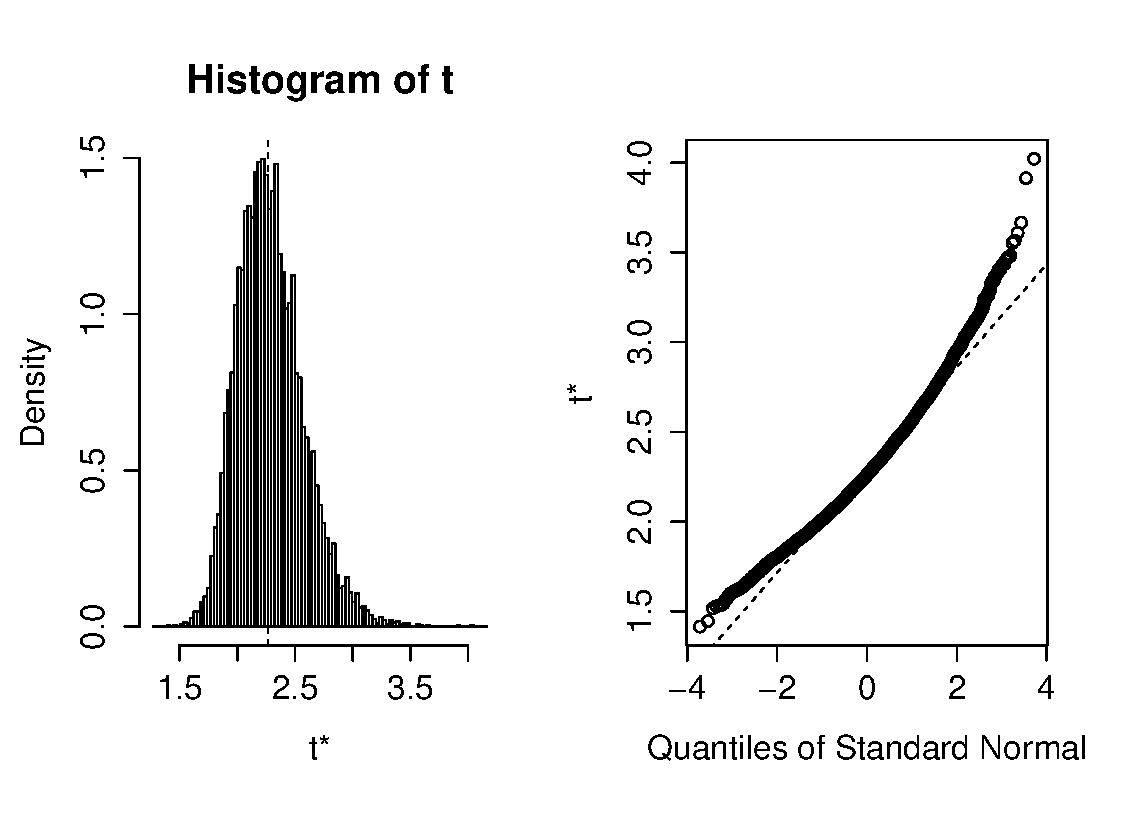
\includegraphics[width = \textwidth]{x0-bootstrap}
%   \includegraphics[width = \textwidth]{boot}
%   \caption{\textit{Left} Histogram of bootstrap replicates, a vertical line indicates the position of the original estimate $\widehat{x}_0$. \textit{Right} Normal Q-Q plot of the bootstrap replicates.}
%   \label{fig:x0-bootstrap}
% \end{figure}

\begin{knitrout}
\definecolor{shadecolor}{rgb}{0.969, 0.969, 0.969}\color{fgcolor}\begin{kframe}
\begin{alltt}
\hlcom{# Bootstrap calibration intervals. In general, nsim should be as large as }
\hlcom{# reasonably possible (say, nsim = 9999).}
\hlstd{boo} \hlkwb{<-} \hlkwd{invest}\hlstd{(mod,} \hlkwc{y0} \hlstd{=} \hlkwd{c}\hlstd{(}\hlnum{309}\hlstd{,} \hlnum{296}\hlstd{,} \hlnum{419}\hlstd{),} \hlkwc{interval} \hlstd{=} \hlstr{"percentile"}\hlstd{,}
              \hlkwc{nsim} \hlstd{=} \hlnum{999}\hlstd{,} \hlkwc{seed} \hlstd{=} \hlnum{101}\hlstd{)}
\hlstd{boo}  \hlcom{# print bootstrap summary}
\end{alltt}
\begin{verbatim}
##  estimate     lower     upper        se      bias 
## 2.2638535 1.8005534 2.9335622 0.2909187 0.0320422
\end{verbatim}
\begin{alltt}
\hlkwd{plot}\hlstd{(boo)}  \hlcom{# plot results}
\end{alltt}
\end{kframe}\begin{figure}
\includegraphics[width=\maxwidth]{figure/x0-bootstrap-1} \caption{\textit{Left} Histogram of bootstrap replicates, a vertical line indicates the position of the original estimate $\widehat{x}_0$. \textit{Right} Normal Q-Q plot of the bootstrap replicates.}\label{fig:x0-bootstrap}
\end{figure}


\end{knitrout}

\section{Summary}

We introduced the \pkg{investr} package for computing point estimates along with inversion and Wald-based confidence intervals for linear and nonlinear calibration problems with constant variance. We also showed how the \pkg{boot} package can be used for constructing approximate $100(1 - \alpha)\%$ calibration intervals, which for convenience, may be incorporated into a future release of \pkg{investr}.  The authors are currently working on extending the package to handle the case of heteroscedastic errors, random coefficient models (e.g., objects of class \code{lme} from the recommended \pkg{nlme} package \citep{pinheiro-nlme-2013}), and even multivariate calibration problems (e.g., objects of class \code{mlm}).

\section{Acknowledgements}

The authors would like to thank two anonymous reviewers and the Editor for their helpful comments and suggestions.

\bibliography{greenwell-kabban}

\address{Brandon M. Greenwell\\
  Air Force Institute of Technology\\
  Wright Ptrsn AFB, OH 45433\\
  USA}\\
\email{brandon.greenwell@afit.edu}

\address{Christine M. Schubert Kabban\\
  Air Force Institute of Technology\\
  Wright Ptrsn AFB, OH 45433\\
  USA}\\
\email{christine.schubertkabban@afit.edu}

\end{article}

\end{document}
